\documentclass[11pt,oneside,letterpaper]{article}

% graphicx package, useful for including eps and pdf graphics
\usepackage{graphicx}
\DeclareGraphicsExtensions{.pdf,.png,.jpg}

% basic packages
\usepackage{color}
\usepackage{parskip}
\usepackage{float}
\usepackage{hyperref}

% text layout
\usepackage{geometry}
\geometry{textwidth=15.25cm} % 15.25cm for single-space, 16.25cm for double-space
\geometry{textheight=22cm} % 22cm for single-space, 22.5cm for double-space

% helps to keep figures from being orphaned on a page by themselves
\renewcommand{\topfraction}{0.85}
\renewcommand{\textfraction}{0.1}

% bold the 'Figure #' in the caption and separate it with a period
% Captions will be left justified
\usepackage[labelfont=bf,labelsep=period,font=small]{caption}

% review layout with double-spacing
%\usepackage{setspace}
%\doublespacing
%\captionsetup{labelfont=bf,labelsep=period,font=doublespacing}

% cite package, to clean up citations in the main text. Do not remove.
\usepackage{cite}
%\renewcommand\citeleft{(}
%\renewcommand\citeright{)}
%\renewcommand\citeform[1]{\textsl{#1}}

% Remove brackets from numbering in list of References
\renewcommand\refname{\large References}
\makeatletter
\renewcommand{\@biblabel}[1]{\quad#1.}
\makeatother

\usepackage{authblk}
\renewcommand\Authands{ \& }
\renewcommand\Authfont{\normalsize \bf}
\renewcommand\Affilfont{\small \normalfont}
\makeatletter
\renewcommand\AB@affilsepx{, \protect\Affilfont}
\makeatother

% notation
\usepackage{amsmath}
\usepackage{amssymb}


\begin{document}

\newgeometry{top=4cm}

Dear Virus Evolution editorial board,

Thank you for your thorough and insightful comments. Please find attached our revised manuscript entitled ``Evolution and rapid spread of a reassortant A(H3N2) virus that predominated the 2017-2018 influenza season''.  This is an update to submission VEVOLU-2019-010. The editorial assessment identified seven major revisions, in addition to minor points raised by individual reviewers.

Point-by-point review responses are attached.

Sincerely,\\
Barney Potter

\newpage

\section*{Reviewer responses}

Original comments are in plain text.  Our responses follow in \textbf{bold}.

\section*{Reviewer 1}
\subsection*{Major comments}
1. The authors used ML tree reconstruction and comparison of tree incongruency to detect the reassortment event in question. This approach is commonly used, however, it entirely relies on visual subjective assessment of the taxa movement in the trees. Sometimes this can be difficult, especially in the cases of complex segment reassortments and little genetic evolution. Although the main conclusion seems to be supported by these trees, it would be nice if this reassortment event was confirmed by another more objective method. GiRaF method (Nagarajan N et al.Nucleic Acids Res. 2011 Mar;39(6):e34) relies on Bayesian statistics of reassortment probability based on numerous tests of phylogenetic incongruencies, and was developed for influenza specifically. It can determine the origins of different segments with statistical support. This could be one approach the authors can use to confirm this reassortment event and the origins of all the segments in the reassortant virus, and perhaps also get better granularity of the origins.\\

\textbf{This is an excellent suggestion. We performed an analysis using GiRaF which identified what we call A2/re as reassortant. We believe that this strengthens our results, and we have included a supplemental figure illustrating the GiRaF results to show this.}

\begin{quotation}
  ...indicated by the local branch index (LBI) which summarizes recent clade growth (Supplemental Fig.~$?$) $?$.
  This reassortment was verified statistically by use of GiRaF $?$, which confirms the strains present in the A2/re clade and those in the matched NA clade as being part of a reassortment event ($conf = 0.99$, Supplemental Fig.~$?$).
\end{quotation}

\begin{figure*}[!h]
    \begin{center}
    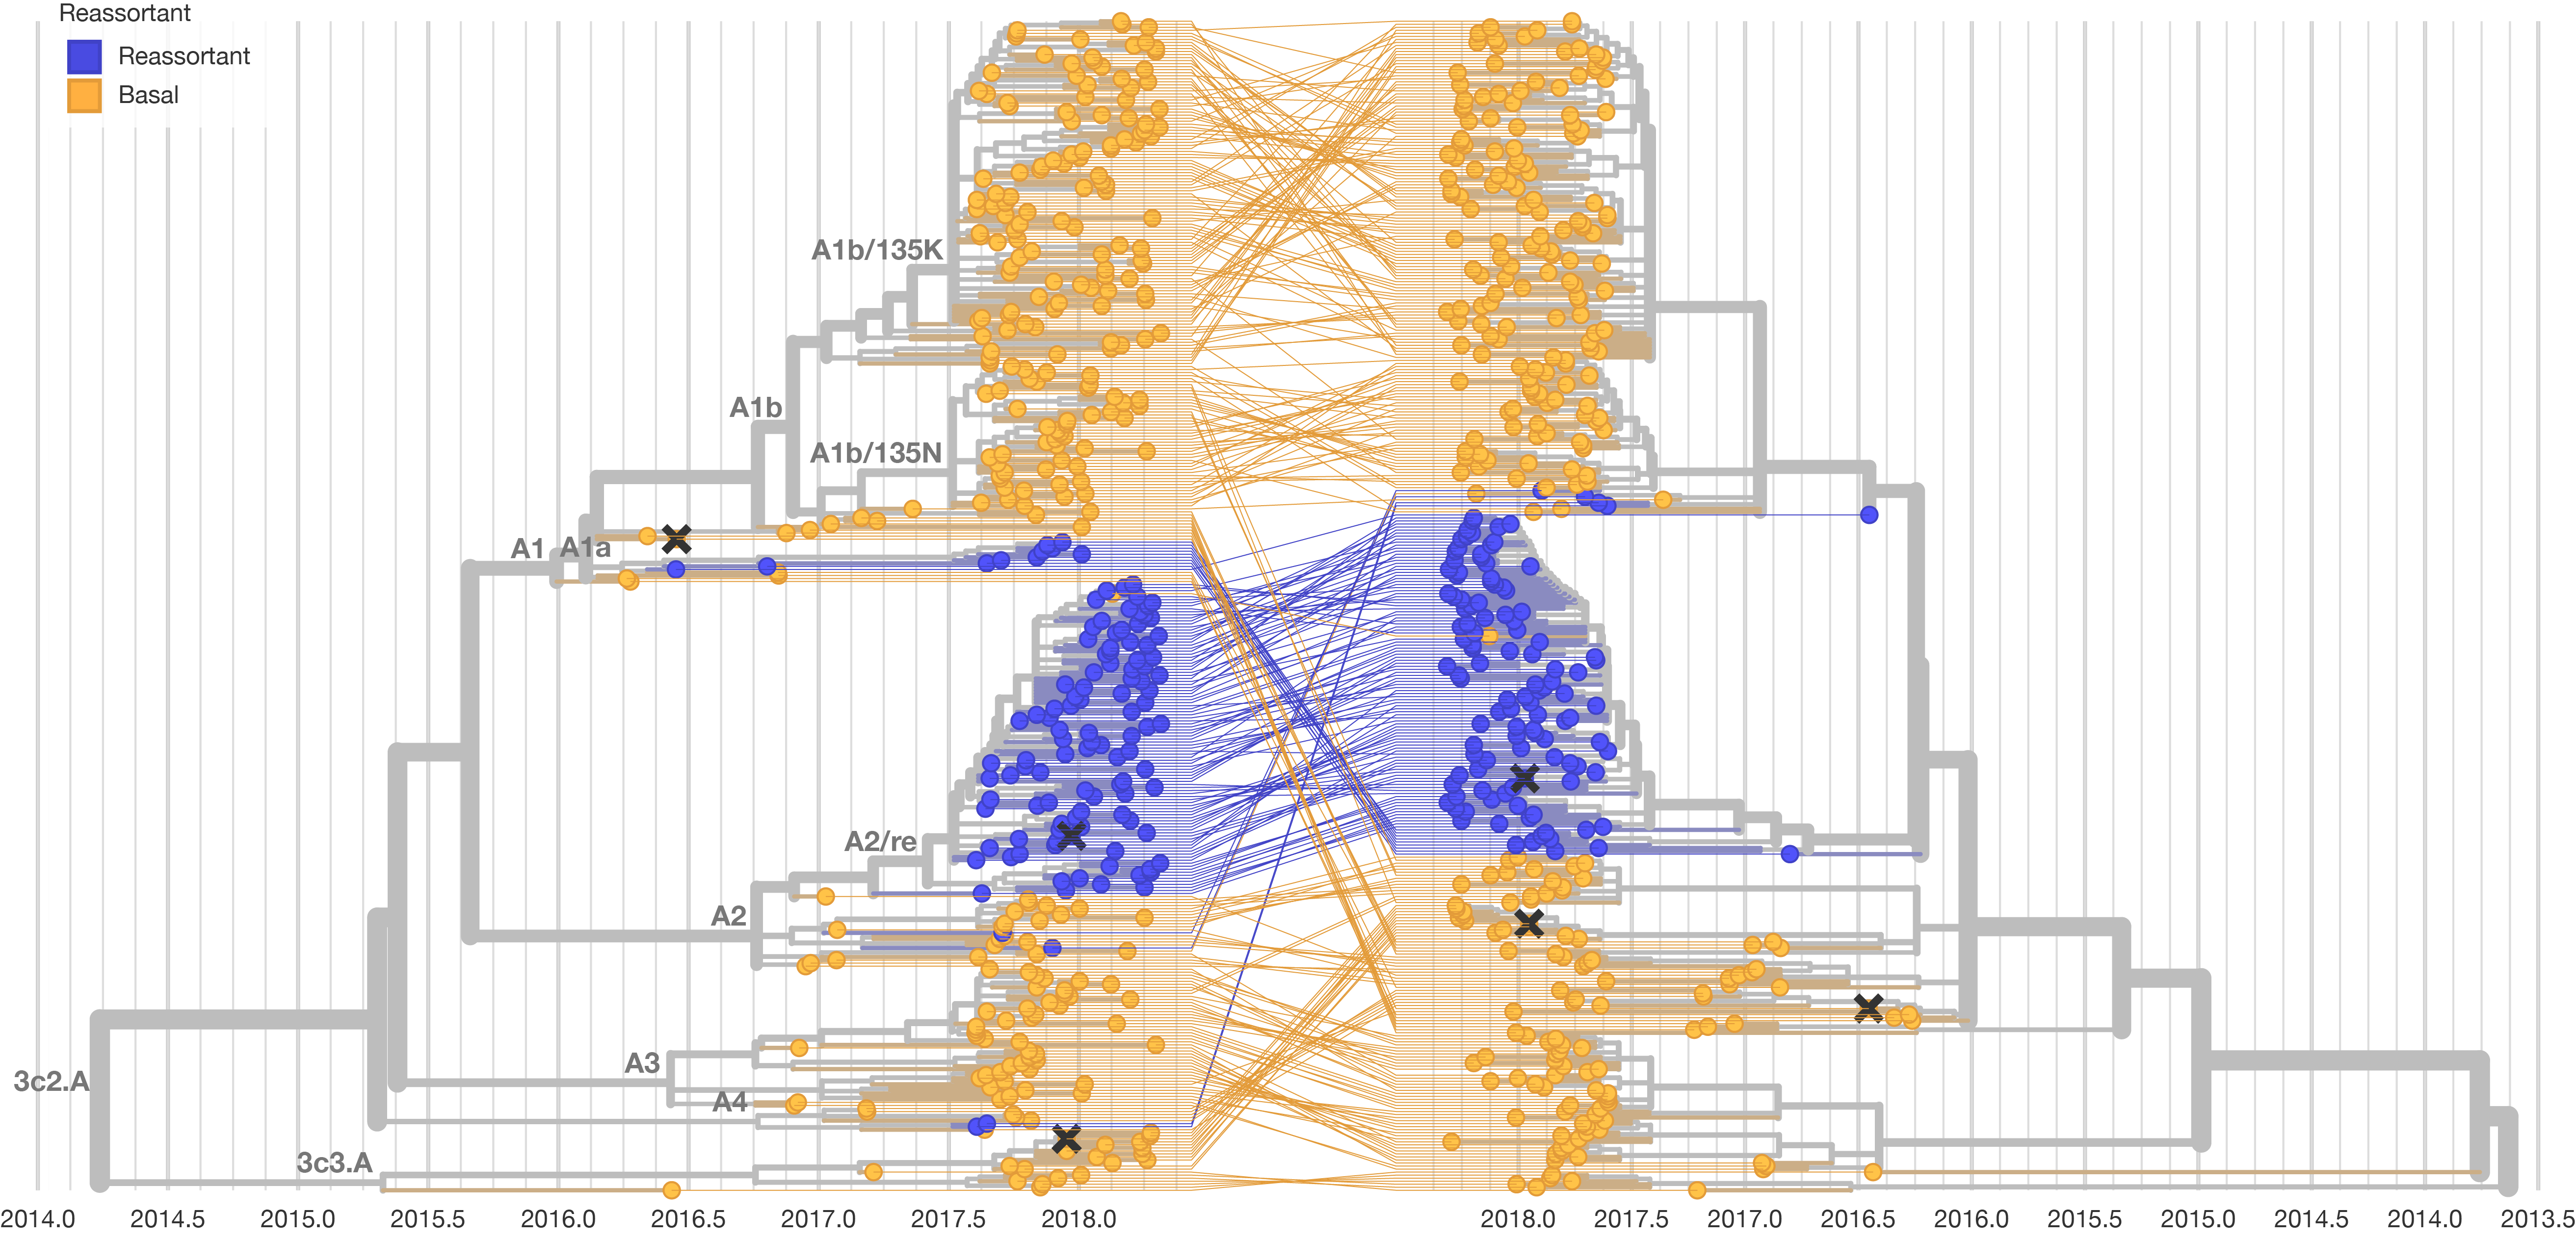
\includegraphics[width=0.75\textwidth]{../manuscript/in-progress/texfiles/figures/giraf_reassortment_results.png}
    \end{center}
    \caption{Tangle tree matching the phylogenies of HA and NA, colored by reassortment status as measured by GiRaF. This coloring shows all tips determined to be part of the reassortment (blue) from both the HA and NA trees.}
    \label{sup_fig:giraf}
\end{figure*}

2. The authors suggest that recurrent changes in the position HA:135 are most probably due to adaptation. There are several ways to measure selective pressure and convergent evolution, and those could be used to analyze if any positive selection pressure exists for this specific position, or any other positions for that matter. These simple and fast analyses might give further insight into the evolution of influenza, including the possible selective pressures in the reassortant virus population (all segments). This might point to residues that may have been important for the increased epidemiologic potential of this variant.\\

\textbf{Thank you for this suggestion. When trying to detect signatures of selection in influenza, we find that traditional $dN/dS$ ratios can often be misleading due to recurrent mutations. One example of this is at the site HA:160, where we see frequent transitions from T to K scattered throughout the phylogeny that do not lead to sustained transmission. This site, when measured by $dN/dS$, shows a strong signature for positive selection, however we believe that this is misleading---particularly when comapred against other mutations that seem to be more beneficial such as at site HA:135. We instead find it more appropriate to observe which mutations rise to high frequency or fixation, rather than their measured $dN/dS$ ratios to determine which high-frequency mutations we should consider as selective in origin. Because this is an important distinction in methodology we have updated the text to reflect this. We have added the results of $dN/dS$ analysis using SLAC, and we have highlighted the repeated T to K transitions at site HA:160 in a supplemental figure to support this.}

\begin{quotation}
  Clade A1 emerged in 2015 and represented the majority of influenza A(H3N2) viruses in the 2016-2017 season.
  Most viruses in this clade differ from the previous vaccine virus (A/Hong Kong/4801/2014) by amino acid substitutions in HA (N121K, N171K, I406V, and G484E).
  Clade A1 further diversified into two subclades now named A1a and A1b.
  These are distinguished by the amino acid substitutions HA:G479E and HA:K92R,H311Q, respectively.
  Further rapid evolution took place within A1b which split into two subclades defined by the HA amino acid substitutions E62G,R142G,T135K, and T135N.
  The recurrent changes at position 135 (including a loss of a putative glycosylation) suggest an adaptive origin of this rapid evolution.
  It is difficult to empirically show that mutations in the HA segment are selected for through $dN/dS$ metrics, as these methods can be convoluted by high numbers of transitions that do not spread further.
  One example of this is at site HA:160, which shows signatures of positive selection when analyzed by SLAC $?$, but this seems to be driven by frequent, unsuccessful mutations rather than by positive selective pressure (Supplemental Table~$?$, Supplemental Fig.~$?$).
  To circumvent this issue, we instead measure focus on mutations that fix or rise to high frequency to determine adaptive origin.
  In the past year A1b has out-competed A1a.
\end{quotation}

\begin{table}[h]
  \caption{Sites showing signatures of positive selection in HA as determined by $dN/dS$ analysis. Site 160 in particular shows evidence of positive selection when analyzedy by this method.}
  \begin{center}
    \begin{tabular}{ccccccc}
    Codon & Partition & S     & N      & dS    & dN     & Selection detected? \\
    53    & 1         & 1.000 & 13.000 & 1.312 & 5.812  & Pos. p = 0.095      \\
    128   & 1         & 0.000 & 8.000  & 0.000 & 4.000  & Pos. p = 0.039      \\
    160   & 1         & 2.000 & 36.000 & 2.058 & 17.807 & Pos. p = 0.000      \\
    193   & 1         & 1.000 & 12.000 & 1.285 & 5.400  & Pos. p = 0.112      \\
    197   & 1         & 0.000 & 6.000  & 0.000 & 3.997  & Pos. p = 0.084      \\
    198   & 1         & 0.000 & 11.000 & 0.000 & 6.209  & Pos. p = 0.007      \\
    214   & 1         & 1.000 & 12.000 & 1.007 & 5.979  & Pos. p = 0.040      \\
    261   & 1         & 1.000 & 7.000  & 0.938 & 5.967  & Pos. p = 0.047
    \end{tabular}
  \end{center}
  \label{sup_tab:hyphy_results}
\end{table}

\begin{figure*}[!h]
    \begin{center}
    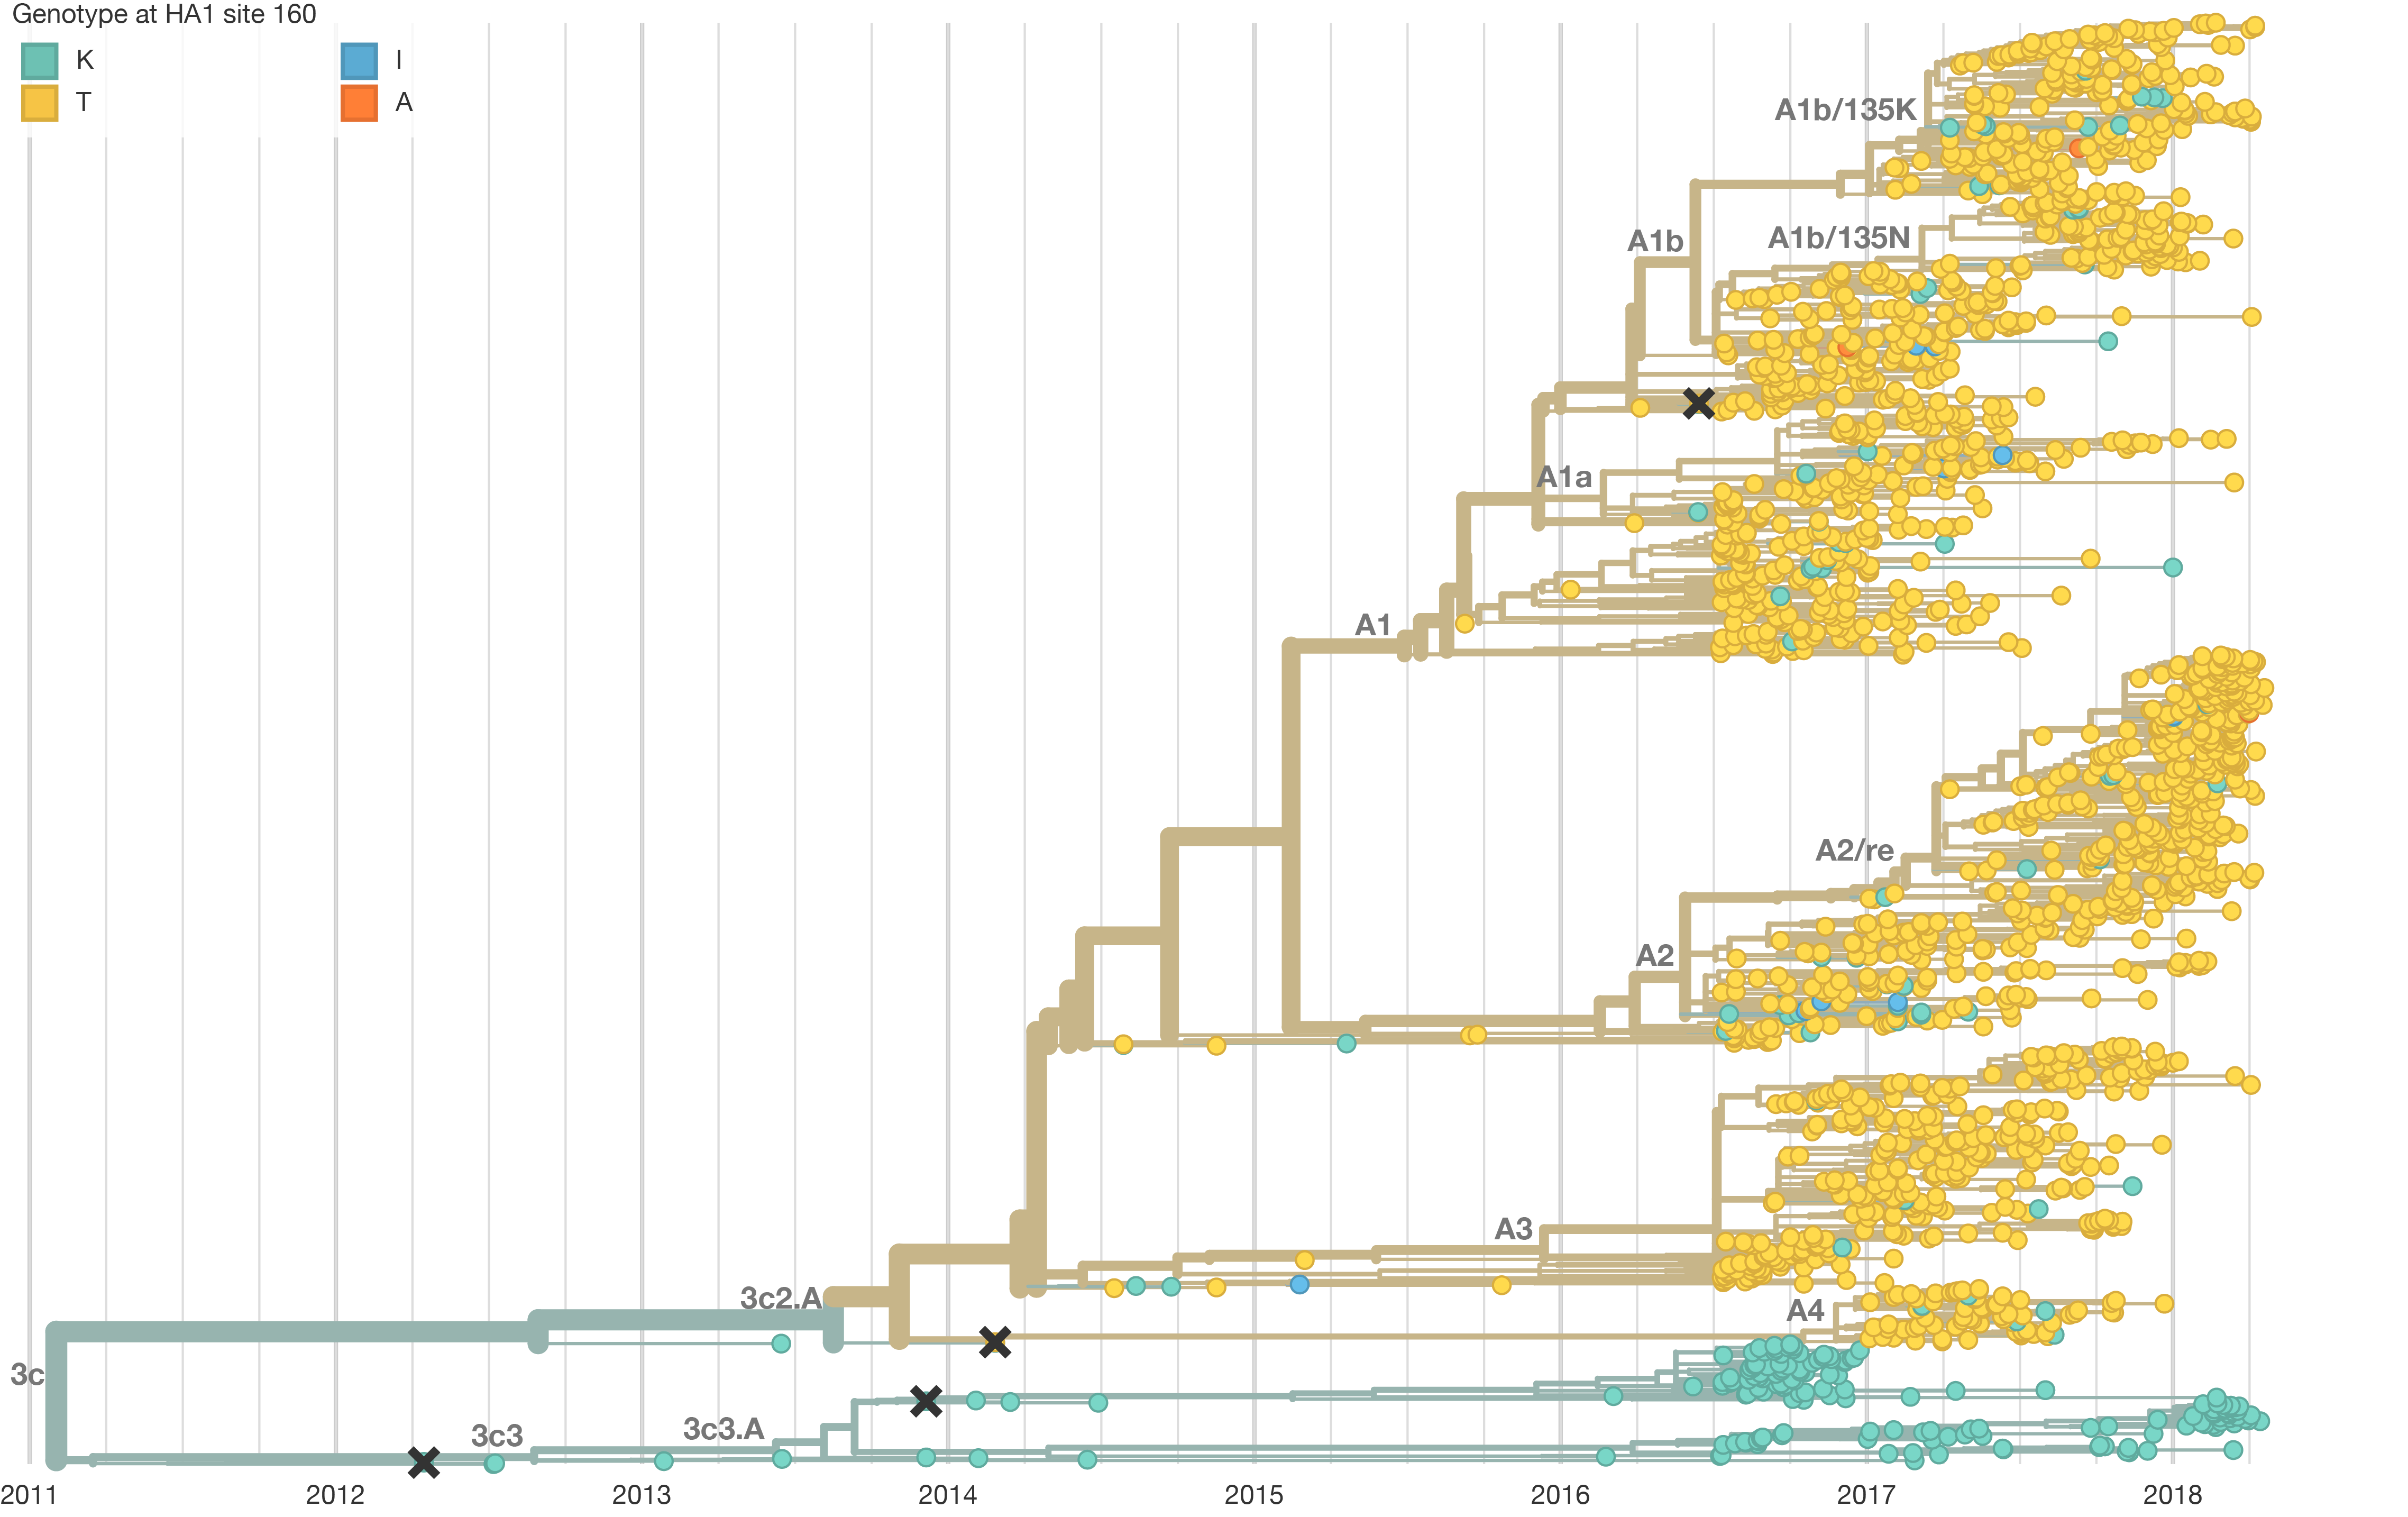
\includegraphics[width=0.75\textwidth]{../manuscript/in-progress/texfiles/figures/ha1160_tree.png}
    \end{center}
    \caption{Phylogeny of HA colored by genotype at site HA:160. The frequent recurrent mutations of T to K, without any sustained growth suggest that this mutation is not adaptive, despite showing evidence of positive selection when analyzed by $dN/dS$ methods.}
    \label{sup_fig:ha1160}
\end{figure*}

3. In the section: Genome reassortment events among circulating viruses leads to A2/re genotype, authors describe a discrete trait phylogeographic model was used to determine the geographic origins of the reassortant virus. This approach was not described in the materials and methods section, so this should be added.\\

4. The geographic origins through phylogeography are determined based on what is available in the used data. Since this analysis was performed on the subsampled dataset there could be missing geographic information that would have changed the results. This is especially true for influenza which experiences less geographical clustering than other RNA viruses. These limitations should be highlighted.\\

\textbf{Thank you for pointing this out, as it is a very important limitation. While we believe that our subsampling method should not introduce geographic bias to the analysis, this is nonetheless important for us to point out. Since our analyses define the reassortant virus as North American based on the bulk of its growth being in North America we still feel comfortable keeping this description. We have, however, updated our discussion to bring this to the readers' attention.}

\begin{quotation}
  Hence assigning significance to any specific reassortment event is difficult and the rapid growth of the A2/re genotype might also be driven by other epidemiological factors.
  We also cannot be sure of the geographic origin of this reassortant virus.
  While our subsampling method samples evenly through time and geography---hopefully preventing introduction of geographic bias---we cannot rule out that the reassortment took place somewhere beyond North America, before rising to prominence in North America.
\end{quotation}

5. Are there any statistics for the TMRCA estimates? Only approximate dates were provided in the text. The authors should provide the estimated dates and their confidence intervals.\\

\textbf{Thank you very much for this suggestion, we have updated the text with the HPD ranges for each TMRCA estimate.}

\begin{quotation}
  Temporal phylogenetic analysis places the MRCA of the A2/re genotype in the HA segment between Dec 2016 and Feb 2017 (95\% HPD 2016-12-28 to 2017-02-11) and in the NA segment between Jan 2017 and Mar 2017 (95\% HPD 2017-01-24 to 2017-03-13), suggesting that most likely a reassortment event in Jan or Feb 2017 gave rise to a virus that seeded the rapidly growing population with this genome constellation.
\end{quotation}

6. It is somewhat difficult to understand what the authors are trying to say with the following sentence: To quantify the rise of A2/re viruses, we calculated frequencies of viruses with genotypes HA:131T / NA:329N (ancestral HA, ancestral NA), HA:131T / NA:329S (ancestral HA, derived NA), HA:131K / NA:329N (derived HA, ancestral NA) and HA:131K / NA:329S (derived HA, derived NA- A2/re genotype) (Fig. 4). What is meant by ancestral and derived? Do these correspond the residues found in the different clades (A2 and A1)? A definition of ancestral and derived for this particular case should be added. In addition, why is HA:131 position selected for this analysis specifically? HA from A2 was defined by 3 different substitutions in positions 131, 142, and 261. So it would be useful to better explain why 131 was special. It would be useful to plot the 131 change on the tree in figure 4, just like NA:329 was plotted.\\

\textbf{An excellent point. Our wording and use of the terms ``ancestral" and ``derived" were indeed quite opaque. We have updated the wording of this section to specifically define those terms, as well as to improve clarity.}

\begin{quotation}
  To quantify the rise of A2/re viruses, we calculated frequencies of viruses with four different genotypes corresponding to HA and NA residues that define transitions into the HA and NA clades involved in the reassortment, which we refer to as \textit{ancestral} and \textit{derived}, respectively.
  We define these residue combinations as: HA:131T / NA:329N (ancestral HA, ancestral NA), HA:131T / NA:329S (ancestral HA, derived NA), HA:131K / NA:329N (derived HA, ancestral NA) and HA:131K / NA:329S (derived HA, derived NA- A2/re genotype) (Fig.~4).
  For this analysis, we use only HA:T131K as an identifying mutation for the derived clade, though we can find the same results through using HA1 sites 142 and 261 as all three can be used to define define the transition between the ancestral and derived states of HA---in our case the split of A2 from A1.
  The three former genotypes were observed at frequencies around 10-20\% in 2016, but the A2/re genotype first appeared in February 2017.
\end{quotation}

7. Materials and methods section is very thin. The authors should add at least the following information into the materials and methods section: \\
a.      How were sequences sub-sampled? Was this done randomly (per region and season), or was it informed by something else?\\
b.      What models of evolution were used for the trees?\\
c.      Antigenic analyses/experiments should be described.\\

\textbf{Thank you for this suggestion, the materials and methods section was indeed a a bit sparse. We have addressed these concerns as follows:
\begin{enumerate}
  \item Our subsampling method attempts to sample evenly across geographical location and time--it prioritizes strains for which antigenic data and all eight genomic segments are available
  \item Our trees are constructed according to the Jukes-Cantor model of nucleotide evolution, and have site heterogeneity accounted for by a CAT model, as implemented through FastTree and RAxML
  \item We now explicitly state that our antigenic data were generated by hemagglutination inhibition assay.
\end{enumerate}}

\subsection*{Minor comments}
1. Page 5, line 9: Authors state: “In addition to rising to high levels, the ILI score stayed above 4\% for 10 weeks during the 2017-2018 North American influenza season.” It would be good explaining what this score is (I’m guessing it is referring to the percentage in Figure 1, but this is nowhere called a score), since everything else is nicely described. It kind of comes out of the blue.\\

\textbf{This is a good point. We have removed the word ``score", and instead describe this as the rate of hospital visits for influenza like illness.}

\begin{quotation}
  In addition to rising to high levels, the rate of hospital visits of symptoms of ILI stayed above 4\% for 10 weeks during the 2017-2018 North American influenza season.
\end{quotation}

2. Page 8 line 31: The authors use their own figure as a reference for proof of common intra-subtype reassortment in influenza. I think there are plenty of other studies that have shown this prior to this one. Those should be referred to instead.\\

\section*{Reviewer 2}
\subsection*{Minor comments}
1. Page 4/20, Line 12-14: Give an example of lower severity somewhere else as a comparison with the high severity in the US.\\

2. Page 4/20, Line 45, 46: Give full name for “CDC” and “GISAID”, before introducing abbreviation.\\

\textbf{Thank you for bringing this oversight to our attention. We have added both full names to the text prior to their first use.}

\begin{quotation}
Now nearly all influenza-positive surveillance specimens received by the United States Centers for Disease Control and Prevention (CDC) are sequenced directly using a next generation sequencing (NGS) strategy and submitted to the Global Initiative on Sharing All Influenza Data (GISAID) Epiflu database...
\end{quotation}

3. Page 5/20, Line 13: Why did the authors choose to subsample over a 2-year window, instead of per year?\\

4. Page 6/20, Line 31: “Further rapid evolution of took place”. Remove “of”\\

\textbf{Thank you for this catch! The text is now updated appropriately:}

\begin{quotation}
  Further rapid evolution took place within A1b which split into two subclades defined by the HA amino acid substitutions E62G,R142G,T135K, and T135N.
\end{quotation}

5. Page 7/20, Line 47-50: “We believe that integrating these sources of information to models of influenza evolution will help to predict future influenza genotype growth and us to mitigate the effect of future influenza outbreaks that would otherwise pose great risk to global human health.”. Sentence is too long, perhaps break as: “We believe that integrating these sources of information into models of influenza evolution will help to predict future influenza genotype growth. Furthermore, it would aid mitigating the effect of future influenza outbreaks that would otherwise pose great risk to global human health.”.\\

\textbf{Thank you for this suggestion, we agree that this wording change will help improve the clarity of our message.}

\begin{quotation}
  We believe that integrating these sources of information into models of influenza evolution will help to predict future influenza genotype growth.
  Furthermore, it would aid mitigating the effect of future influenza outbreaks that would otherwise pose great risk to global human health.
\end{quotation}

6. Page 19/22, Figure S1 and S2: Correct the annotation “A1b/135N” which seems to be written twice.\\

7. Page 21/22, Figure S2: Correct the white shadow in the legend that is covering the A1b annotations in the HA tree.\\

\textbf{Thank you for cathing these oversights. We have updated both supplemental figures according to these suggestions.}

\clearpage
\renewcommand{\thefigure}{S\arabic{figure}}

% \bibliography{./../mers-structure}
\begin{figure*}[t!]
    \begin{center}
    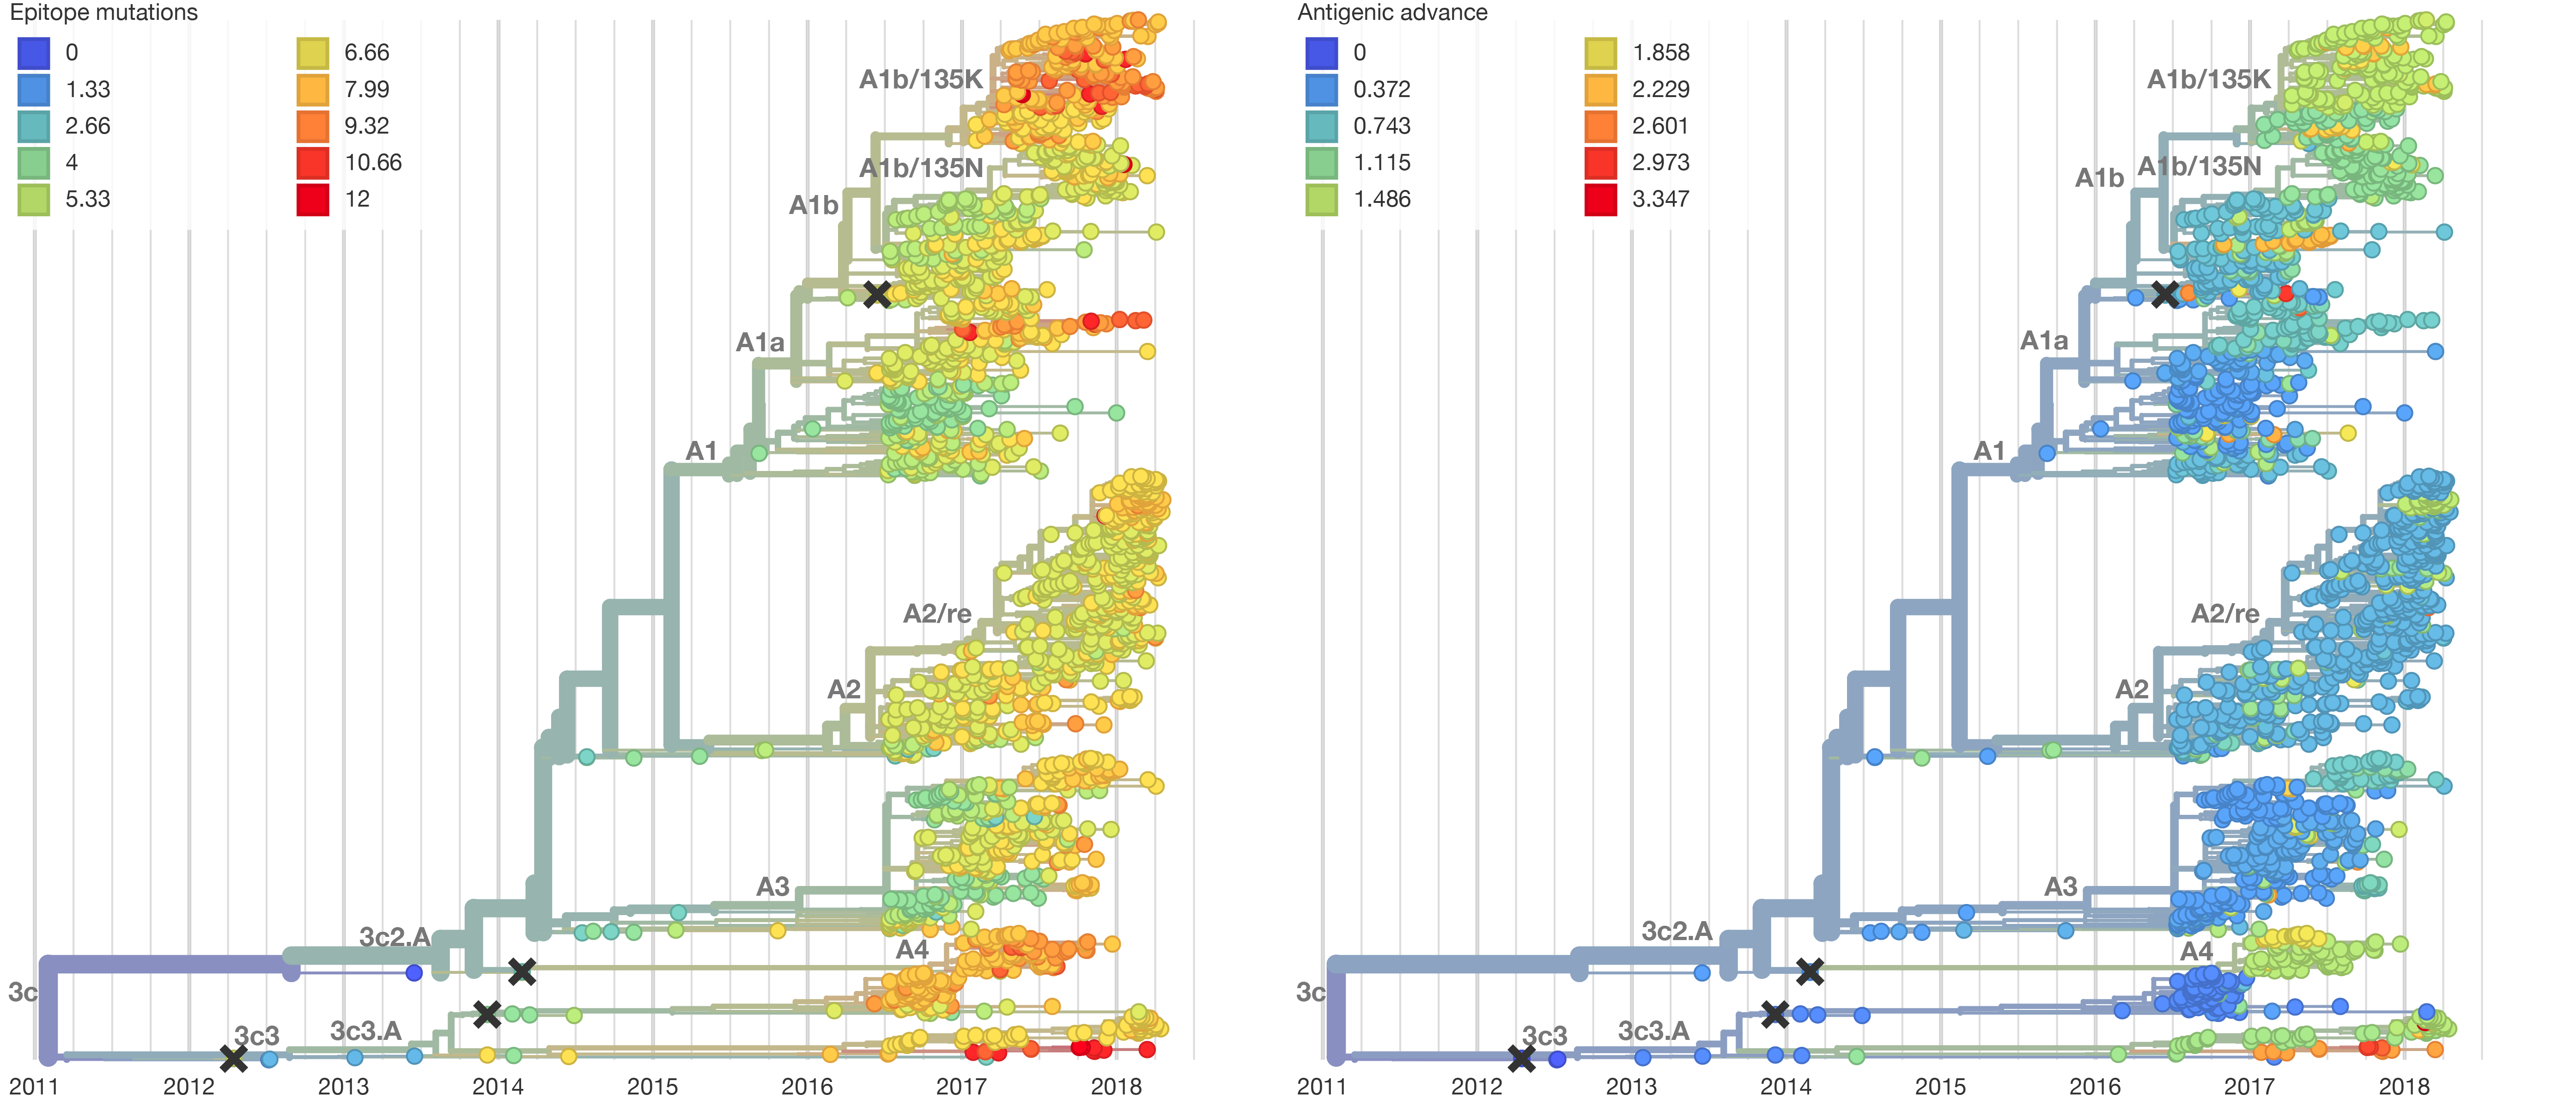
\includegraphics[width=\textwidth]{../manuscript/in-progress/texfiles/figures/epi_aa_trees_high_res.png}
    \end{center}
    \caption{\textit{(left)} Temporally resolved haemagglutinin phylogenetic tree colored by amino acid mutations in epitope sites [38] of HA. \textit{(right)} The same tree, colored by antigenic advance---a measure of how much antigenic drift viruses have undergone based on related viruses' HI titers. Both measures normally indicate that a clade may be prone to grow rapidly, due to increased ability to escape immune pressure. In both trees A2/re does not demonstrate any change from A2, making its sudden growth unusual.}
    \label{sup_fig:epitope_aa}
\end{figure*}

\begin{figure*}[b]
    \begin{center}
    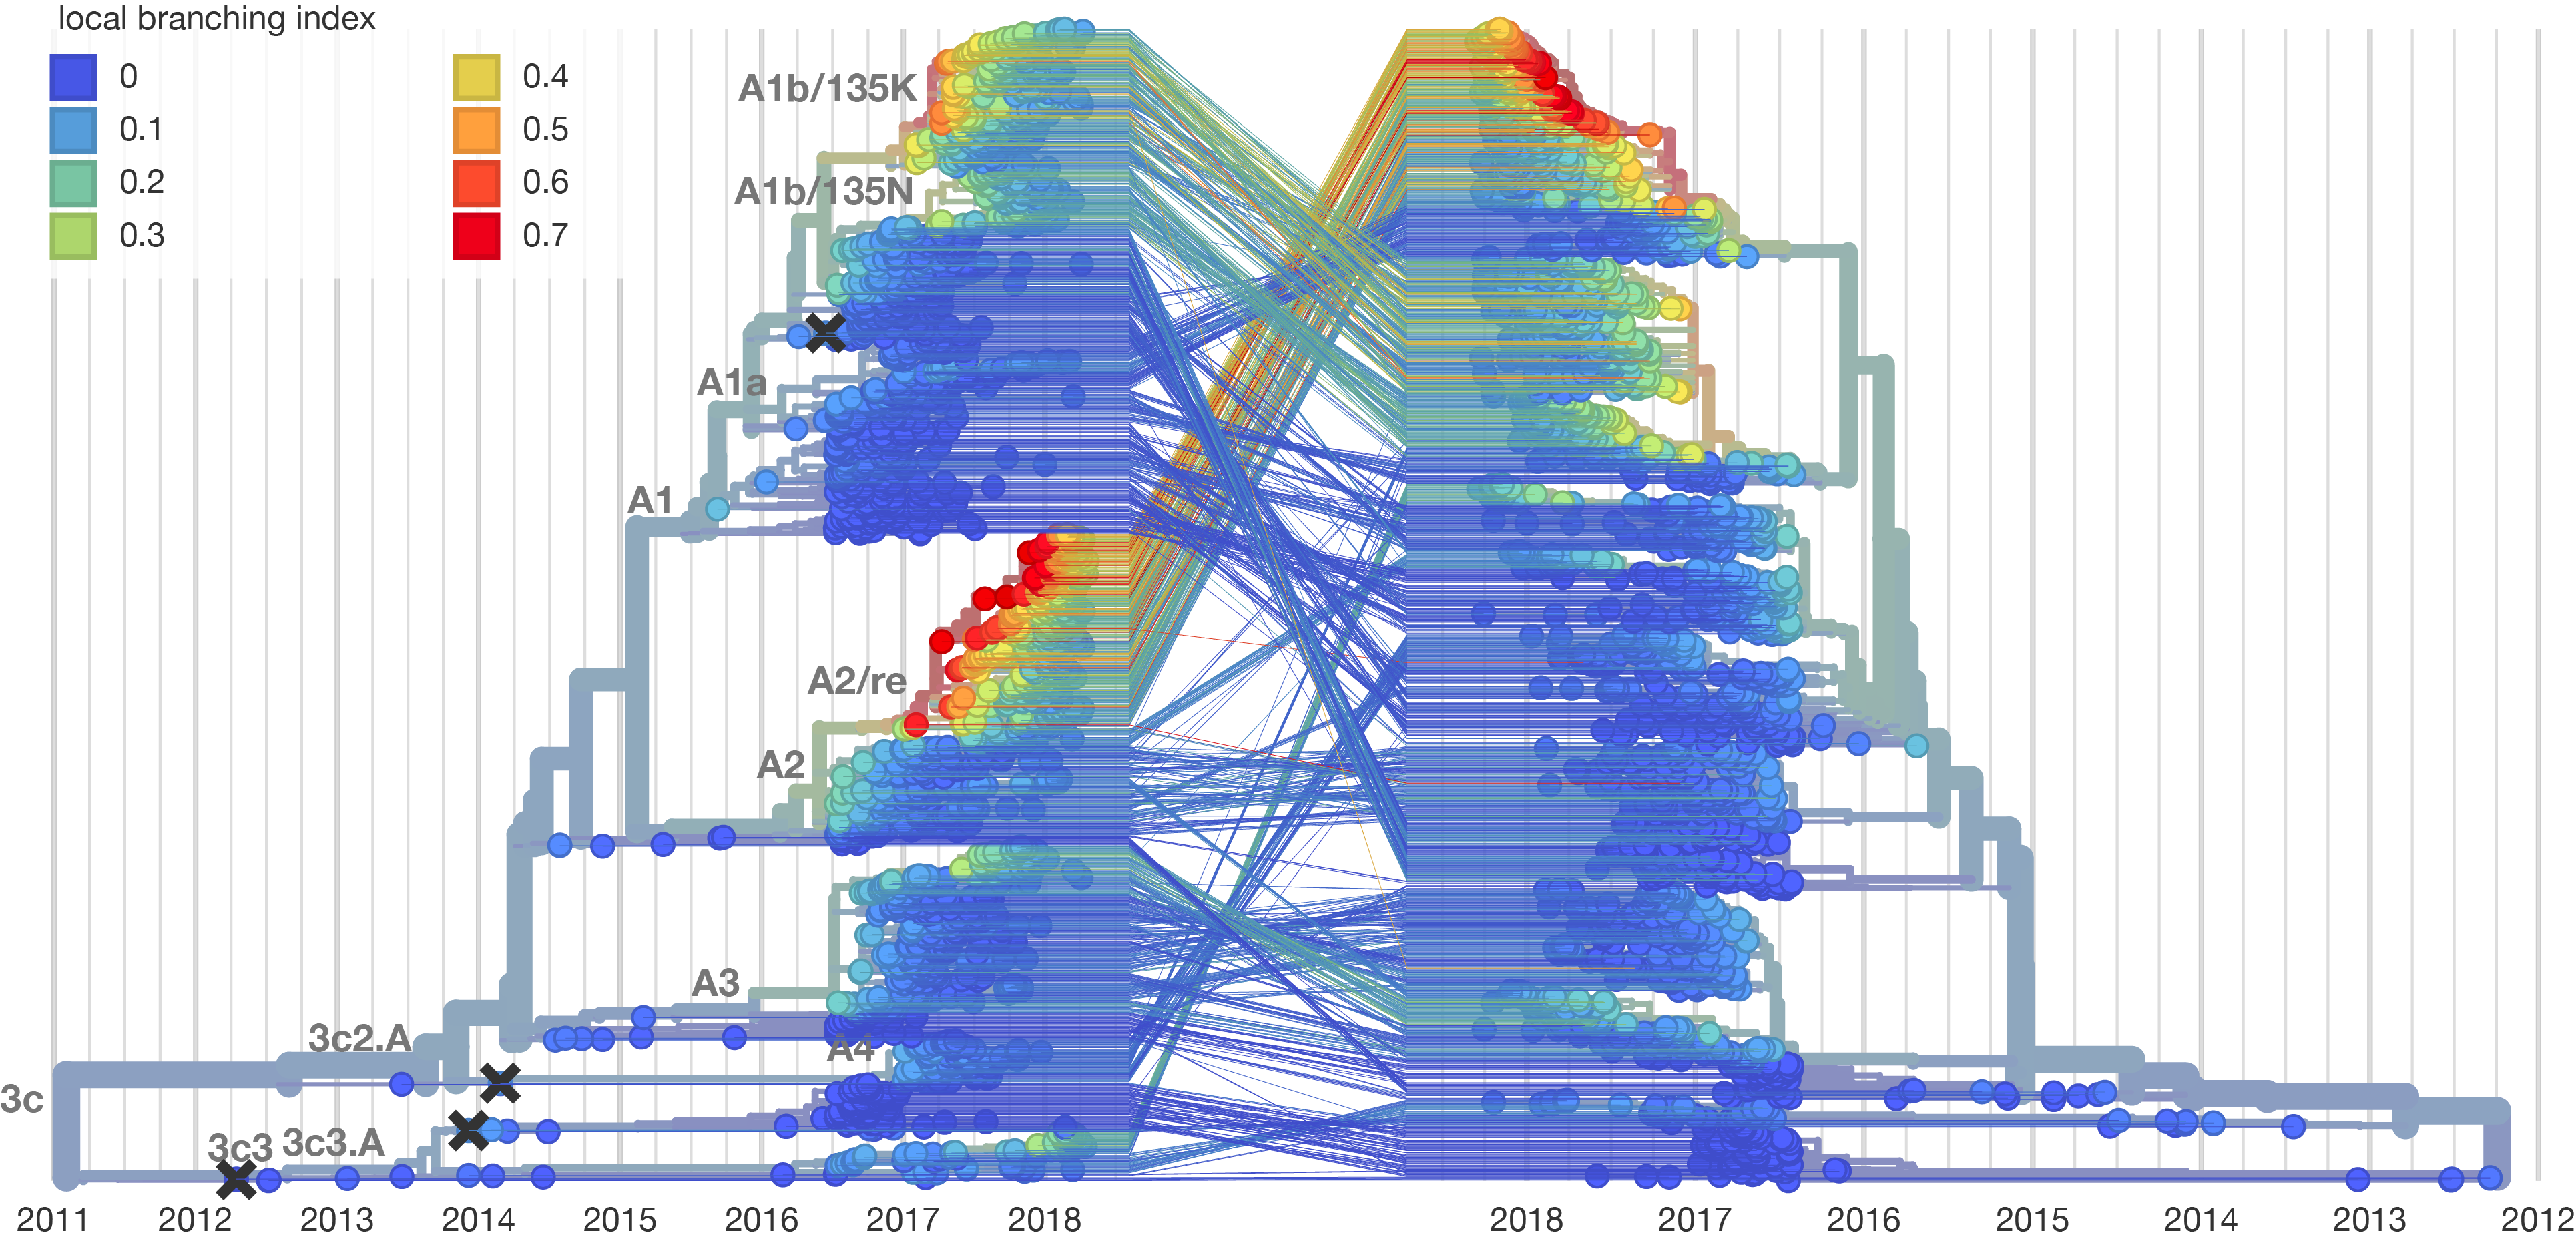
\includegraphics[width=0.85\textwidth]{../manuscript/in-progress/texfiles/figures/ha_na_lbi_high_res.png}
    \end{center}
    \caption{Tangle tree matching phylogenetic trees of HA and NA, colored by local branching index (LBI)---a measure that captures rapid expansion of clades. Here, LBI reveals that there is an inflection point where rapid clade growth begins at the same time that A2/re differentiates from A2 in the HA tree. Similarly, LBI is highest in the matched viruses of the NA tree, indicating that the reassortant virus saw much greater success than either of the background viruses from which it arose.}
    \label{sup_fig:lbi}
\end{figure*}

\end{document}
